\section{One-Factor Short-Rate Model}
The risk-free short rate, r, is sometimes referred to as the instantaneous short rate. 
The concept is used in finance modeling to represent the continuously compounded interest rate for 
short time intervals. The short rate, r, is often modeled using stochastic deferential equations in 
mathematical finance. Some typically models for modeling the short rate is the Vacisek model and the Cox–Ingersoll–Ross model, 
later the Vacisek model will be covered. When pricing derivatives as bonds and options, the price depends on 
the process followed by r in the risk-neutral world \cite{Hull}.
\\\\
As discussed in the section Risk Neutral Measure, $r_t$ can be looked at the locally risk-free 
rate from a continuously compounded bank account $B(t)= \exp \Big[\int_{0}^{t} r(s) ds \Big]$. 
Where the bank account has the dynamic listed in \autoref{bank1} and \autoref{bank2}.
Postulation the considered market is arbitrage-free, with due to the First Fundamental Theorem of Asset Pricing, 
if stating that there exist a probability measure $\QQ$, equivalent to $\PP$, all asset prices discounted by $B(t)$
are $\QQ$-martingales. In other words under the considered market for any T we have that 
\begin{align}
    \frac{P(0,T)}{B(0)} = P(0,T) = \EE^{\QQ} \Big( \frac{P(T,T)}{B(T)}\Big) = \EE^{\QQ} \Big( \frac{1}{B(T)}\Big) 
    = \EE^{\QQ} \Big( \exp \Big[ - \int_{0}^{t}r(s)ds \Big] \Big)
    \label{dist}
\end{align}
where $P(0,T)$ is the price at time zero of the asset and note that $P(T,T)=1$. So \autoref{dist} says that 
the time zero price of the asset are $\QQ$-expectations  of the payoff \cite{Bermudan}.
In other words in a market free of arbitrage, bond prices are determined by the risk-neutral expectations 
of how the short-term interest rate will behave. Because all types of interest rate instruments are based
on bond prices, the entire term structure or zero-coupon curve can be described by the distributional properties
of just one state variable - the short rate \cite{Bermudan}.

\subsection{The Vasicek model}
So all interest rate instruments are fundamentally dependent on bond prices. Understanding the movements of 
these prices is essential for accurately describing the term structure or zero coupon curve. The behavior 
of the short rate, a key variable, underlies this understanding due to its distributional properties.
\\\\
The Vasicek model, introduced by Oldrich Vasicek in 1977, serves as a robust framework to analyze these dynamics.
The Vasicek model is renown for its simplicity and the ease with which it facilitates bond price calculations, 
the model assumes that the short-term interest rate adheres to a mean-reverting stochastic process. This process is characterized 
by parameters that dictate the rate's mean reversion speed, its long-term average level, and its volatility.
The model is used for forecasting how interest rates in the market will develop in the future. The model is a
mathematical result of interest rates and it is a one-factor short rate model and the model is constructed in the 
term of that the evolution of interest rates only depends on stochastic variable.
\\\\
So now a short introducing to the Vasicek model has been covered and the next step is to look closer at the 
mathematical framework of the Vasicek model. The Vasicek model consists of the dynamic of the short rate under the $\PP$-measure
(the real world measure). Where the dynamic of the short rate is governed by a stochastic differential equation. 
The dynamic for the short rate in the Vasicek model is present below in \autoref{vas_dyn} and \autoref{vas_dyn_r0} \cite{Bjork}.
\begin{align}
    d r_t &= \kappa \Big[\theta -r(t)\Big] dt + \sigma d W(t) \label{vas_dyn}\\
    r(0) &= r_0 \label{vas_dyn_r0}
\end{align}
The dynamic for the short rate in \autoref{vas_dyn} is a Ornstein-Uhlenbeck process, which is a type of stochastic 
differential equation that describes the evolution of a mean-reverting behavior. So the process is consisting of a 
tendency to revert towards the mean of the process. This tendency is illustrated in \autoref{fig:vasicek} below, where 
interest rates is simulated using the Vasicek Model for some chosen parameters. Note in \autoref{fig:vasicek}
one simulated path of the short rate is illustrated. Where in \autoref{fig:vasicek-sim} 20 simulated paths are illustrated,
but the same tendency appears. The parameters in the short rate dynamic
$\kappa$, $\theta$ and $\sigma$ are positive constants. Where $\kappa$ represent the mean reversion speed, $\theta$ 
is the long-term average rate, $\sigma$ is the volatility  and $dW(t)$ is a Wiener process \cite{Bermudan}. 

\begin{figure}[h]
    \centering
    \begin{minipage}{0.5\textwidth}
        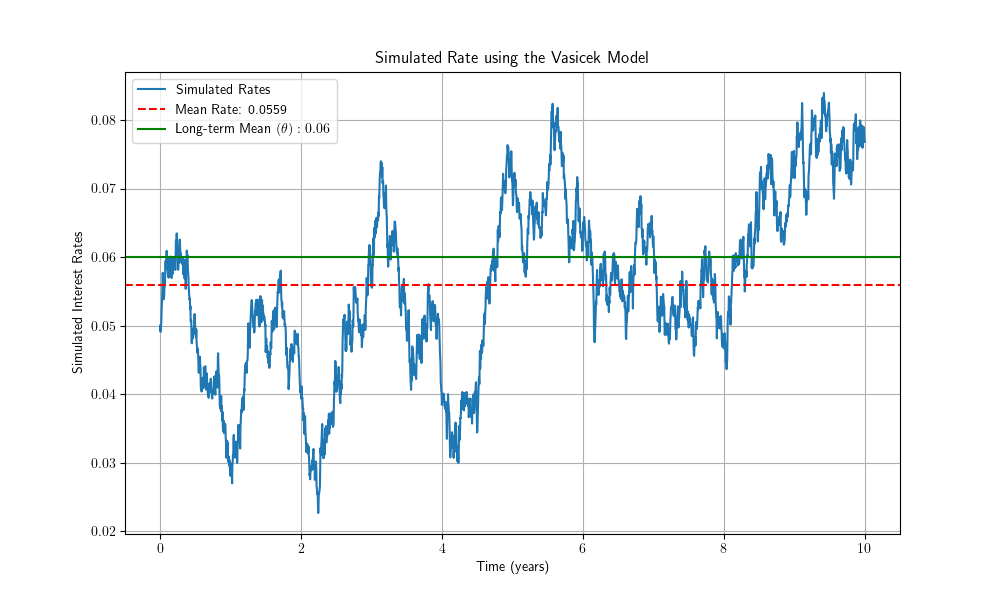
\includegraphics[width=\linewidth]{/Users/nannaingemannohrt/Desktop/master_thesis/main/plots/VasicekModelPlot.png}
        \caption{Plot of one simulated interest rates path \\ using the Vasicek model.}
        \label{fig:vasicek}
    \end{minipage}\hfill 
    \begin{minipage}{0.5\textwidth}
        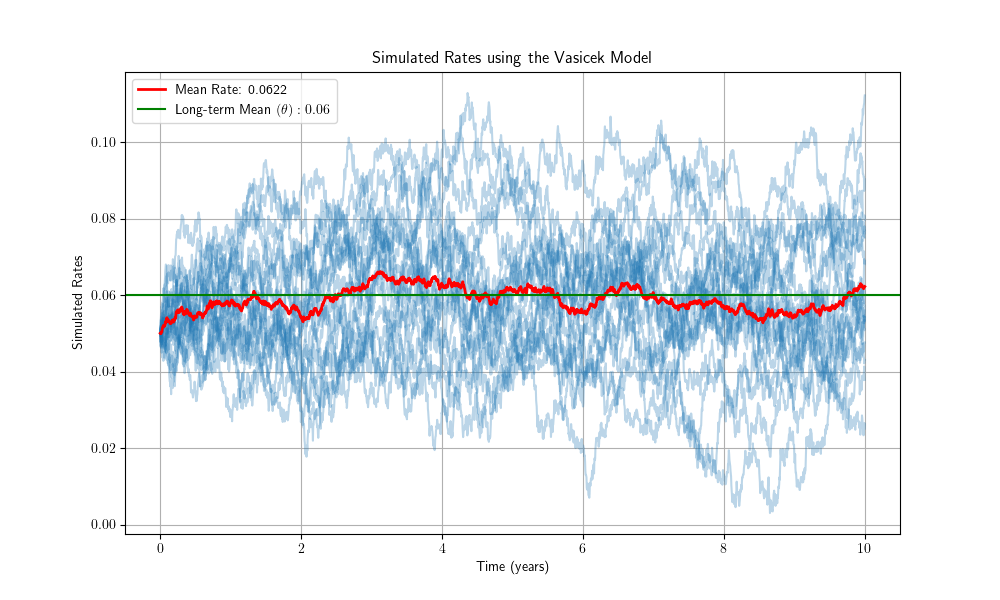
\includegraphics[width=\linewidth]{/Users/nannaingemannohrt/Desktop/master_thesis/main/plots/VasicekModelPlotSIM.png}
        \caption{Plot of 20 simulated interest rates \\ paths using the Vasicek model.}
        \label{fig:vasicek-sim}
    \end{minipage}
\end{figure}

\noindent
\newpage
\noindent
Then we look closer at the dynamic of the short rate in \autoref{vas_dyn}. Which can be rearranged and integrated
to express the short rate, $r(t)$, as a function of its value at any prior time point s, 
so we have to have that $s < t$ \cite{Bermudan}. 
\begin{align}
    d r_t &= \kappa \left[\theta - r(t)\right] dt + \sigma d W(t) \label{line_14} \\
    d r(t) &= k \theta dt - k r(t) dt + \sigma d W(t),  \\
    d r(t) + k r(t) dt &= k \theta dt + \sigma d W(t), \\
    e^{kt} d r(t) + k e^{kt} r(t) dt &= e^{kt} k \theta dt + e^{kt} \sigma d W(t), \\
    \frac{d}{dt} \left( e^{k t} r(t) \right) &= e^{k t} \frac{d}{dt} r(t) + k e^{k t} r_t dt, \\
    d\left( e^{k t} r(t) \right) &= e^{k t} dr(t) + k e^{k t} r_t dt, \\
    \int_s^t d \left( e^{ku} r(u) \right) &= k \theta \int_s^t e^{ku} du + \sigma \int_s^t e^{ku} d W(u), \\
    e^{kt} r(t) - e^{k s} r(s) &= \frac{k \theta}{k} \left( e^{kt} - e^{ks} \right) + \sigma \int_s^t e^{ku} d W(u), \\
    r(t) &= r(s) e^{-k(t-s)} + \theta \left( 1 - e^{-k(t-s)} \right) + \sigma \int_s^t e^{-k(t-u)} d W(u). \label{line_22}
\end{align}
From \autoref{line_14} to \autoref{line_22} the expression for the short rate in the Vasicek model is integrated, but first
rearranged the terms i the stochastic differential equation. Then both sides of the equation are multiplied by the 
integrating factor $e^{\kappa t}$ to facilitate integration. Next both sides is integrated from s to t. The result of the
integration showing the change in the interest rate, r, over time, adjusted by the integrating factor. The final 
expression in \autoref{line_22} for the interest rate, $r(t)$, at time t, showing how it depends on the initial rate, $r(s)$,
the mean-reverting term and the stochastic term \cite{Bermudan}. 

\begin{figure}[h]
    \centering
    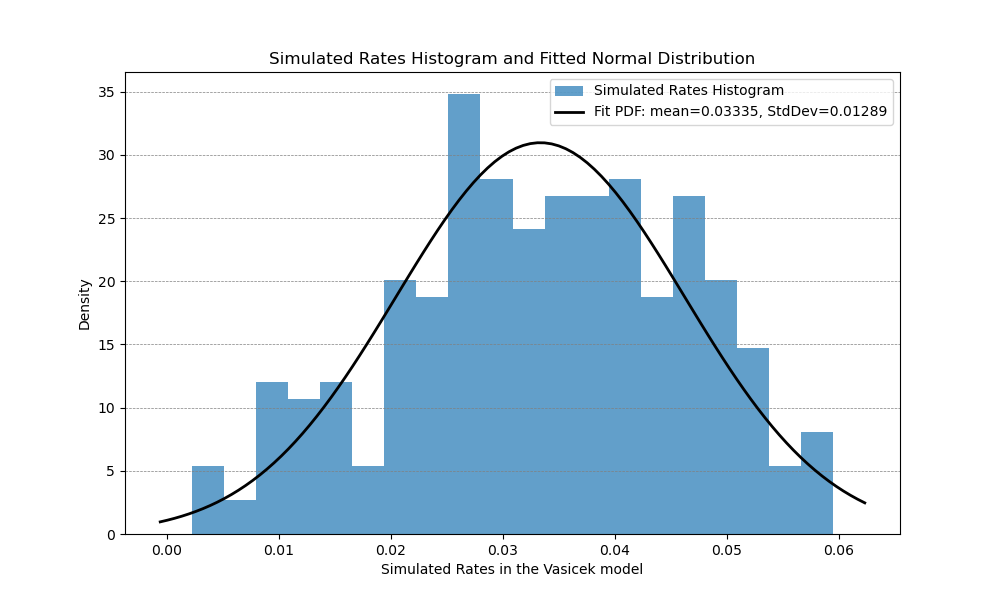
\includegraphics[width=0.7\textwidth]{/Users/nannaingemannohrt/Desktop/master_thesis/main/plots/NormalDistributionPlot.png}
    \caption{Histogram of one simulated interest rates path using the Vasicek model.}
    \label{fig:rates:hist}
\end{figure}